In this section we document the 2D ($m_{ll}, m_T$) templates used in this analysis.  

\subsection{Signal and background templates}
Figure~\ref{fig:hww2d_lowmass_0j}-\ref{fig:bkg2d_lowmass_0j} show the 
templates used for the 0-Jet bin for the signal and background processes. 

%%%%%%%%%%%%%%%%%%%%%%%%%%%%%%%
\begin{figure}[!hbtp]
\centering
\subfigure[mH(120)]{
\centering
\label{subfig:h120_0j}
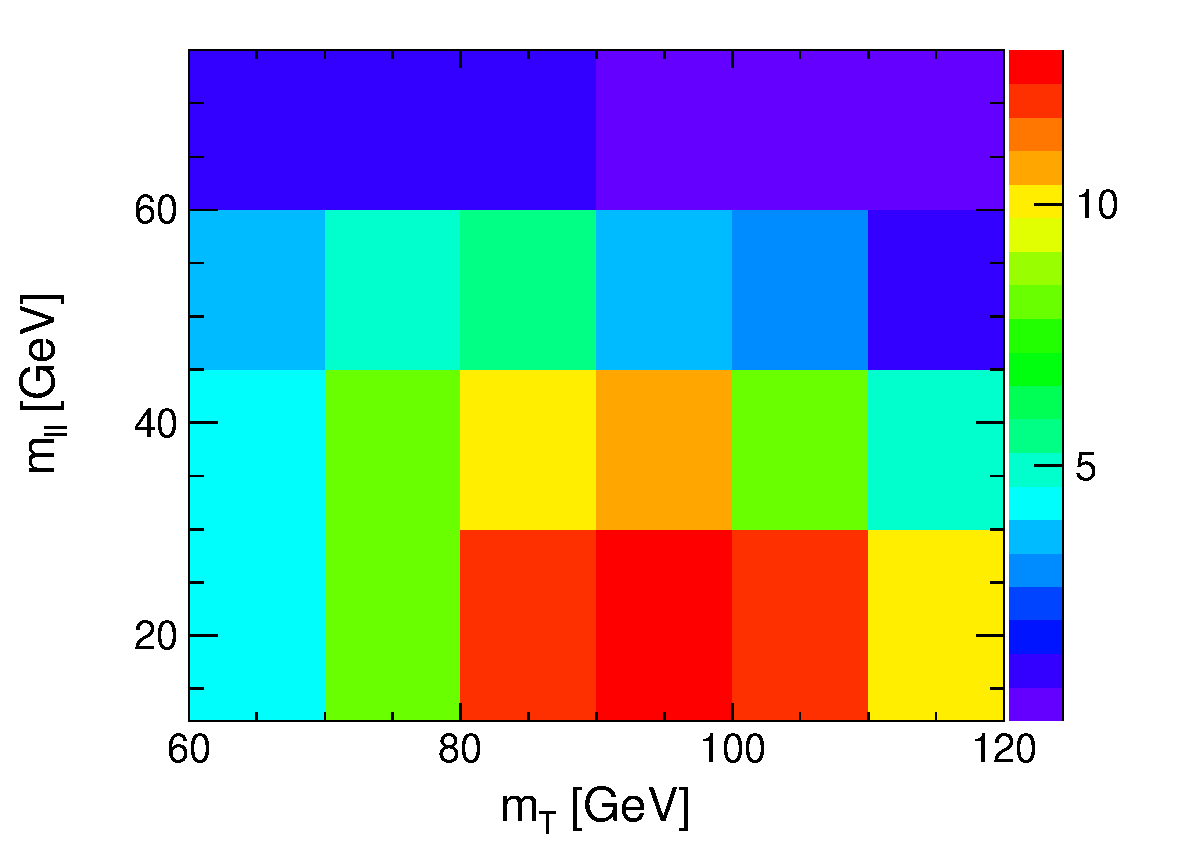
\includegraphics[width=.3\textwidth]{figures/mtvsmll_hww_120_0j.pdf}
}
\subfigure[mH(125)]{
\centering
\label{subfig:h125_0j}
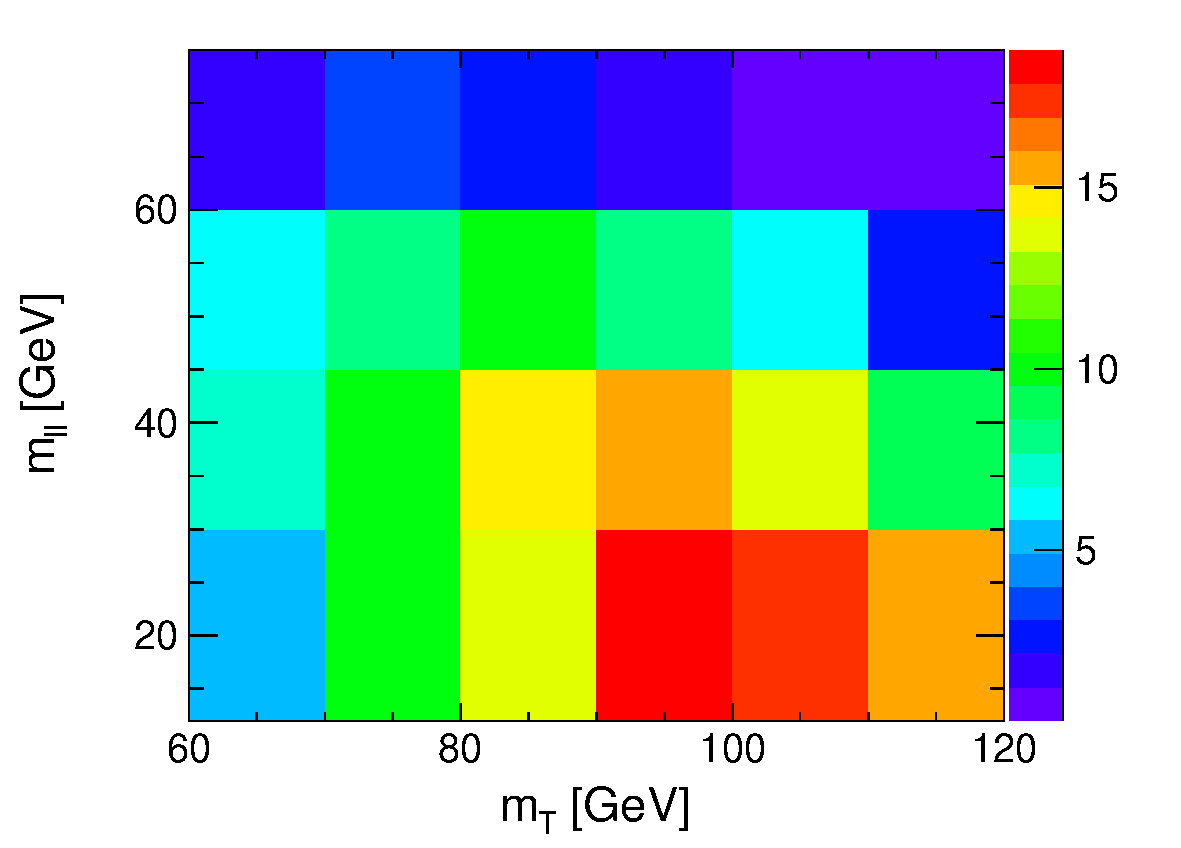
\includegraphics[width=.3\textwidth]{figures/mtvsmll_hww_125_0j.pdf}
} 
\subfigure[mH(130)]{
\centering
\label{subfig:h130_0j}
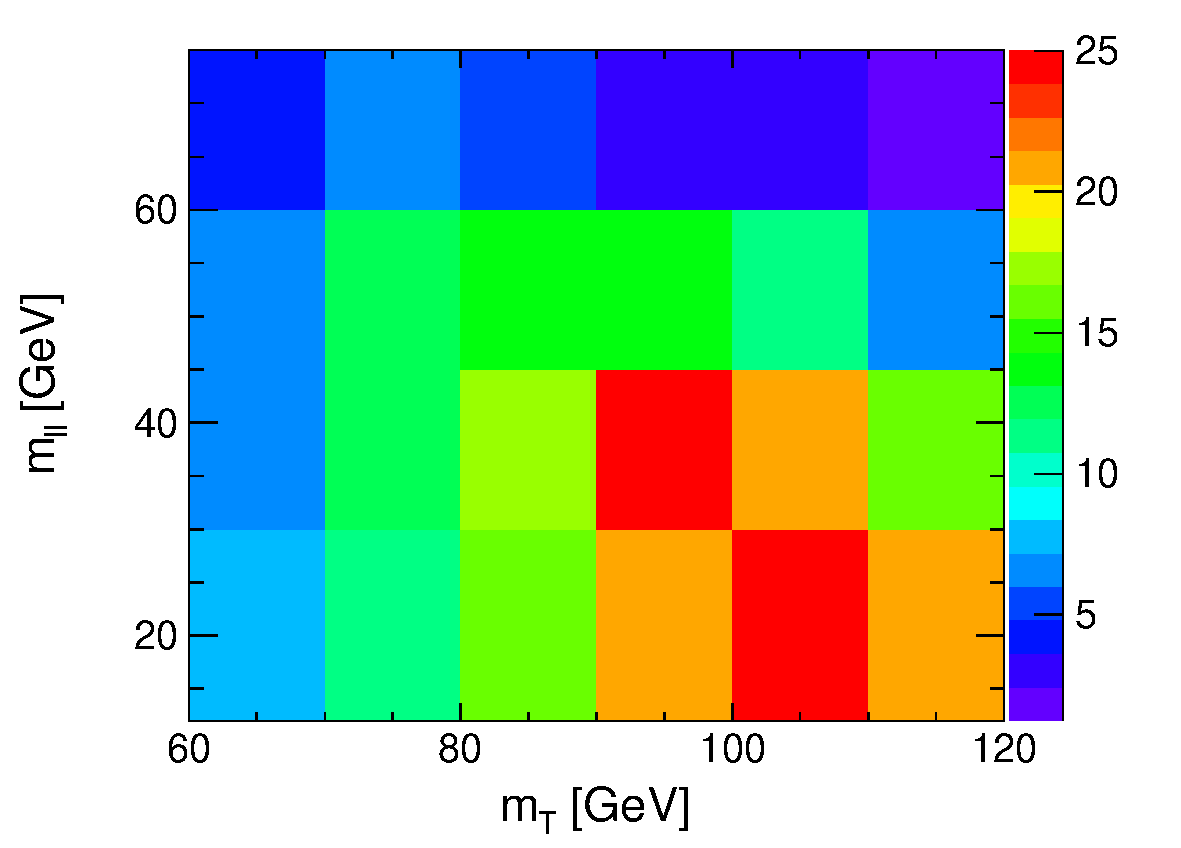
\includegraphics[width=.3\textwidth]{figures/mtvsmll_hww_130_0j.pdf}
} \\
\subfigure[mH(140)]{
\centering
\label{subfig:h140_0j}
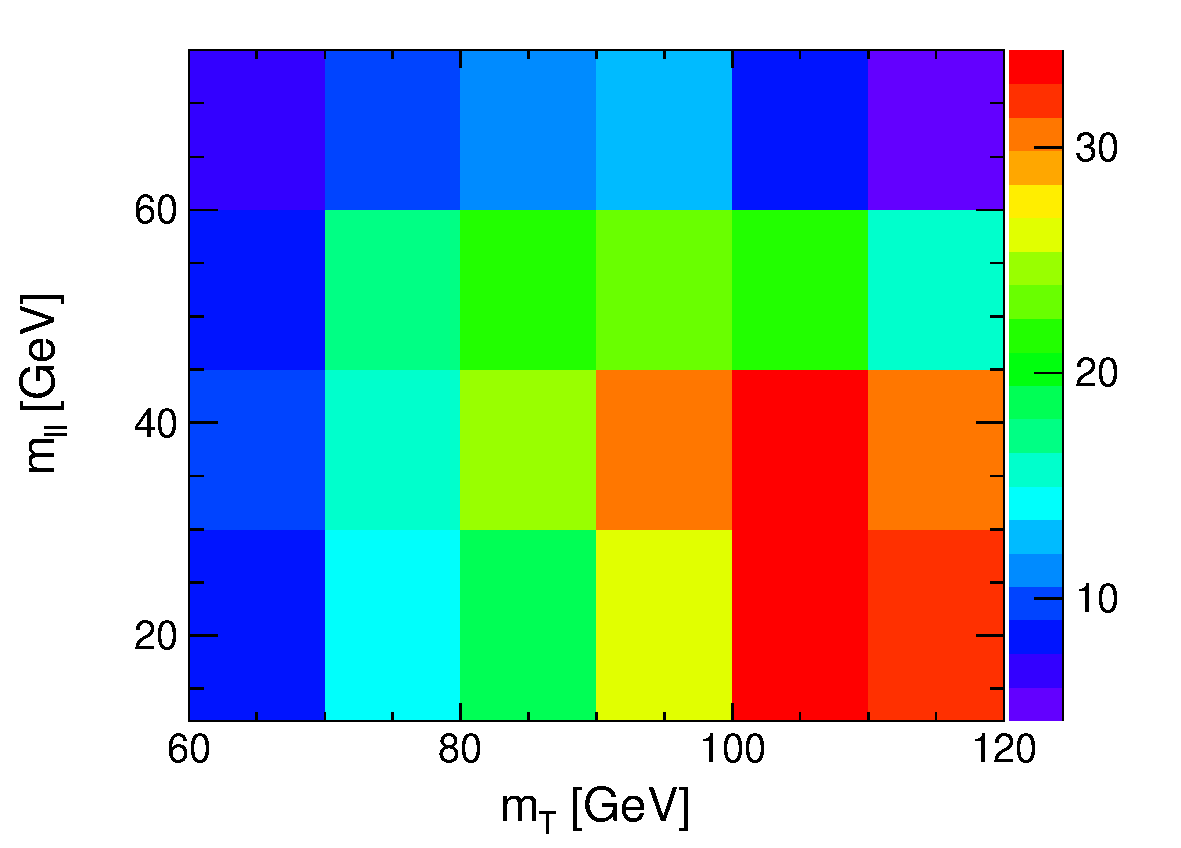
\includegraphics[width=.3\textwidth]{figures/mtvsmll_hww_140_0j.pdf}
}
\subfigure[mH(150)]{
\centering
\label{subfig:h150_0j}
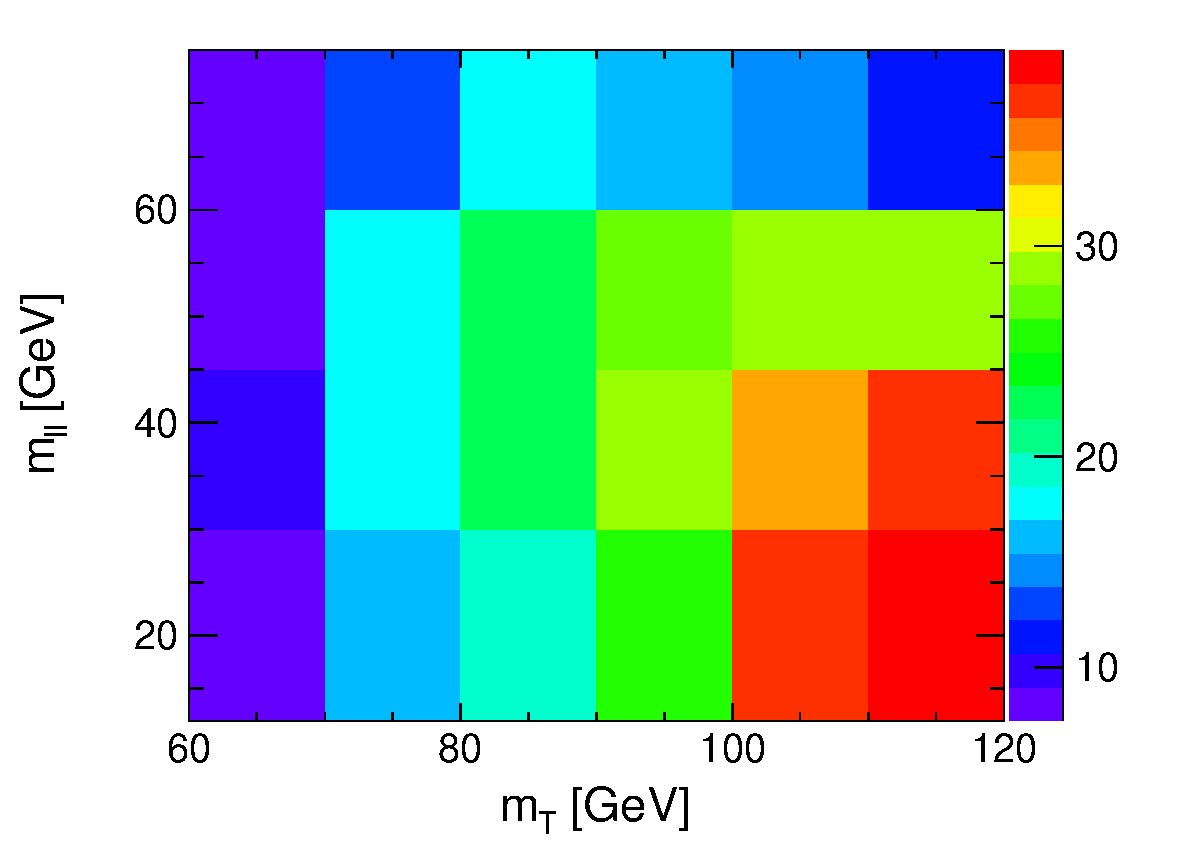
\includegraphics[width=.3\textwidth]{figures/mtvsmll_hww_150_0j.pdf}
} 
\subfigure[mH(160)]{
\centering
\label{subfig:h160_0j}
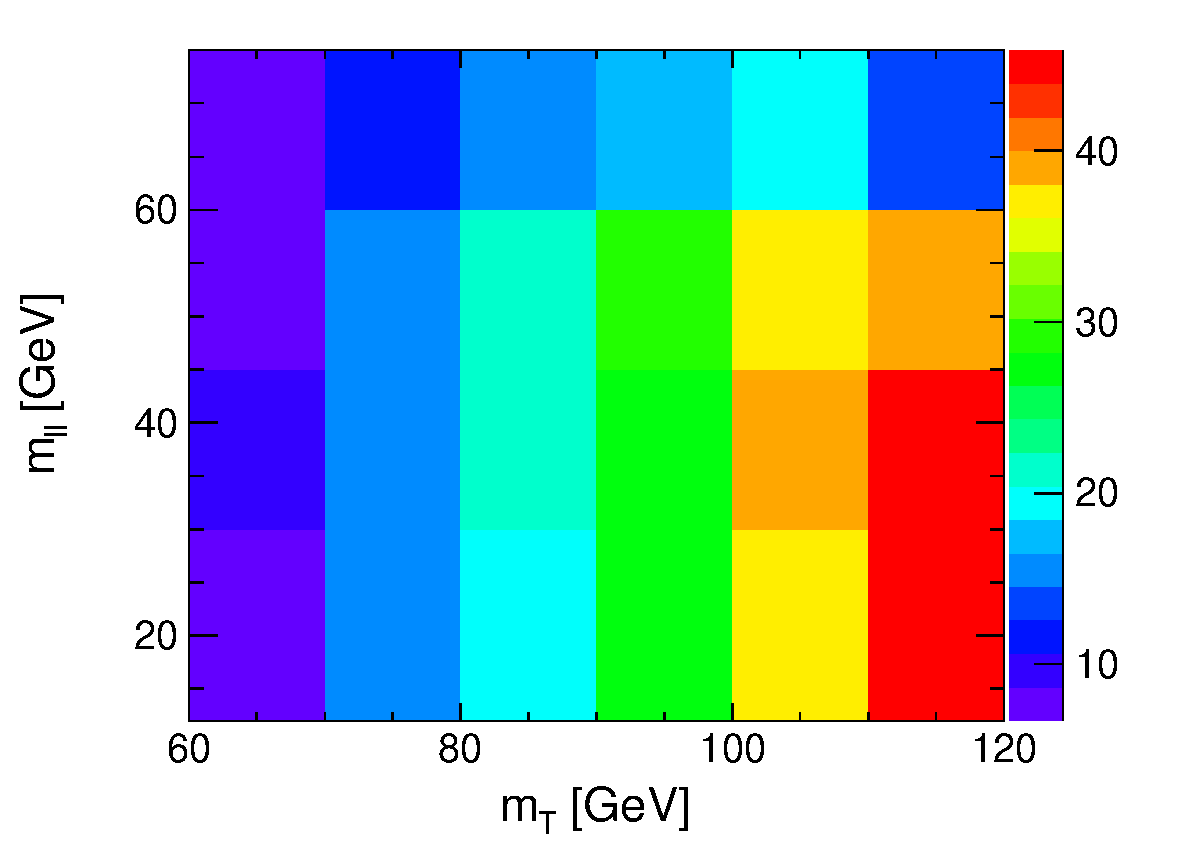
\includegraphics[width=.3\textwidth]{figures/mtvsmll_hww_160_0j.pdf}
} \\
\subfigure[mH(170)]{
\centering
\label{subfig:h170_0j}
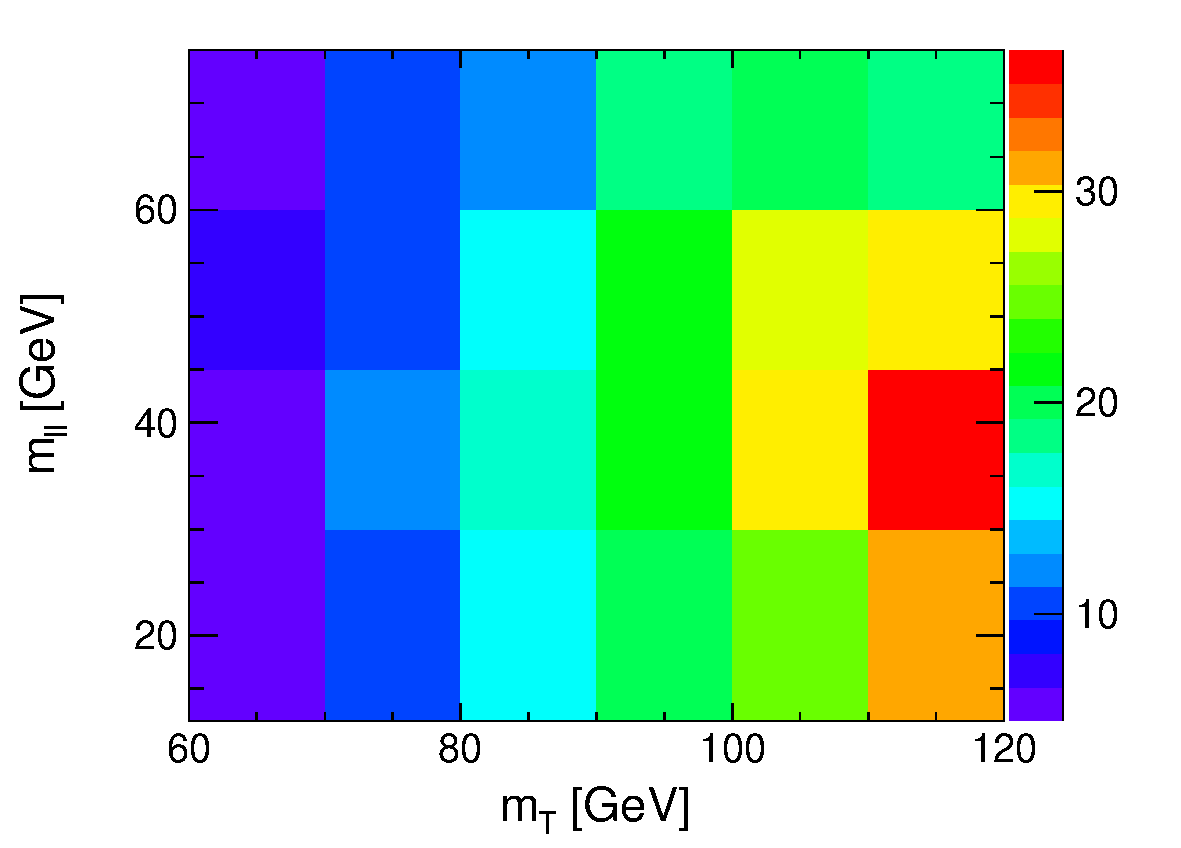
\includegraphics[width=.3\textwidth]{figures/mtvsmll_hww_170_0j.pdf}
} 
\subfigure[mH(180)]{
\centering
\label{subfig:h180_0j}
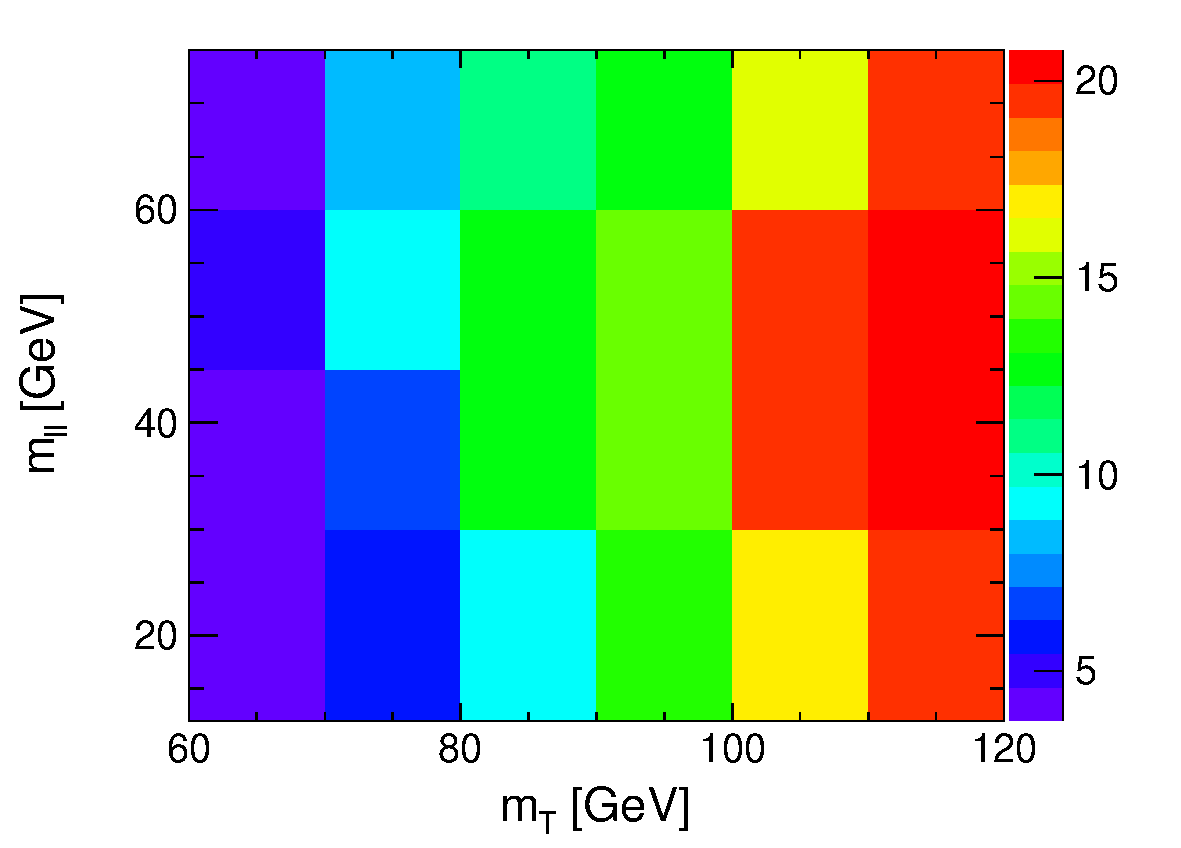
\includegraphics[width=.3\textwidth]{figures/mtvsmll_hww_180_0j.pdf}
} 
\subfigure[mH(190)]{
\centering
\label{subfig:h190_0j}
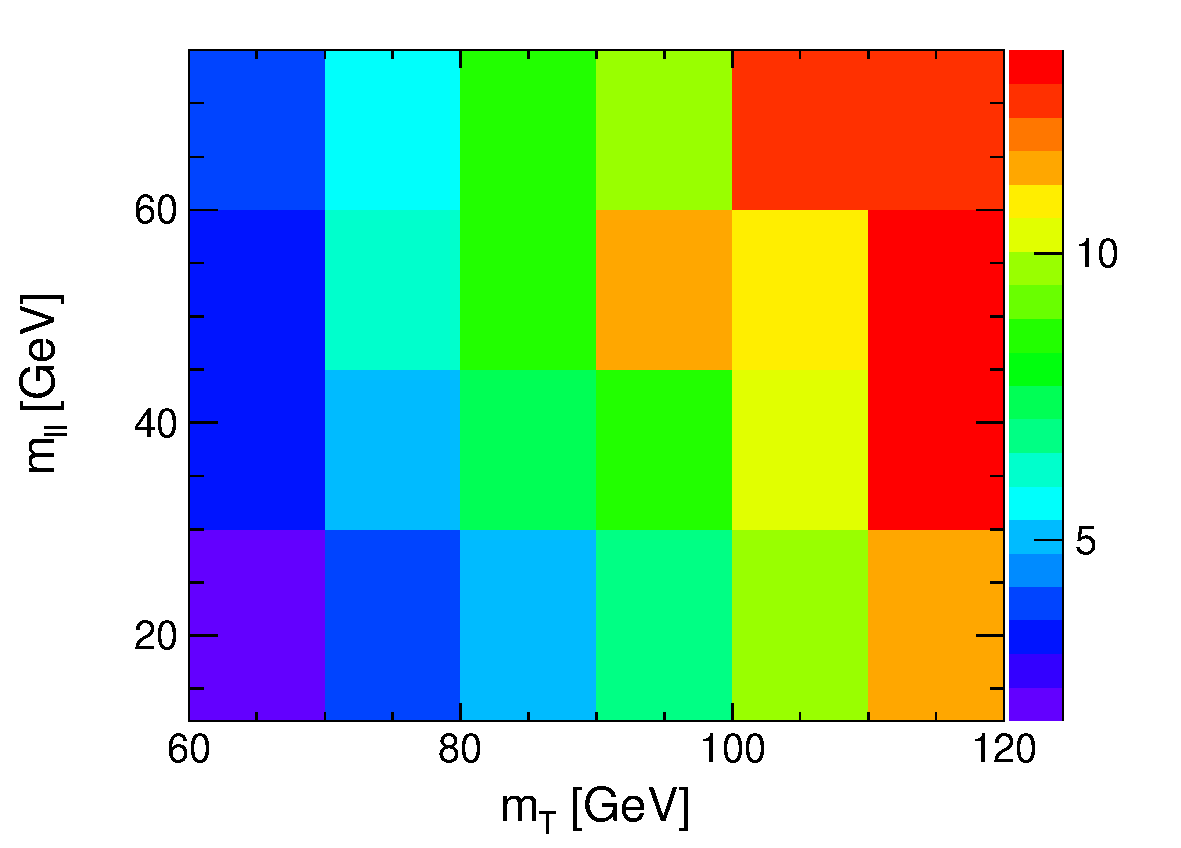
\includegraphics[width=.3\textwidth]{figures/mtvsmll_hww_190_0j.pdf}
} \\
\caption{ The 2D ($m_{ll}, m_T$) templates for the $gg\to H\to WW$ in the 0-Jet bin with low mass region.}
\label{fig:hww2d_lowmass_0j}
\end{figure}
%%%%%%%%%%%%%%%%%%%%%%%%%%%%%%%


%%%%%%%%%%%%%%%%%%%%%%%%%%%%%%%
\begin{figure}[!hbtp]
\centering
\subfigure[$qq\to WW$]{
\centering
\label{subfig:qqww_0j}
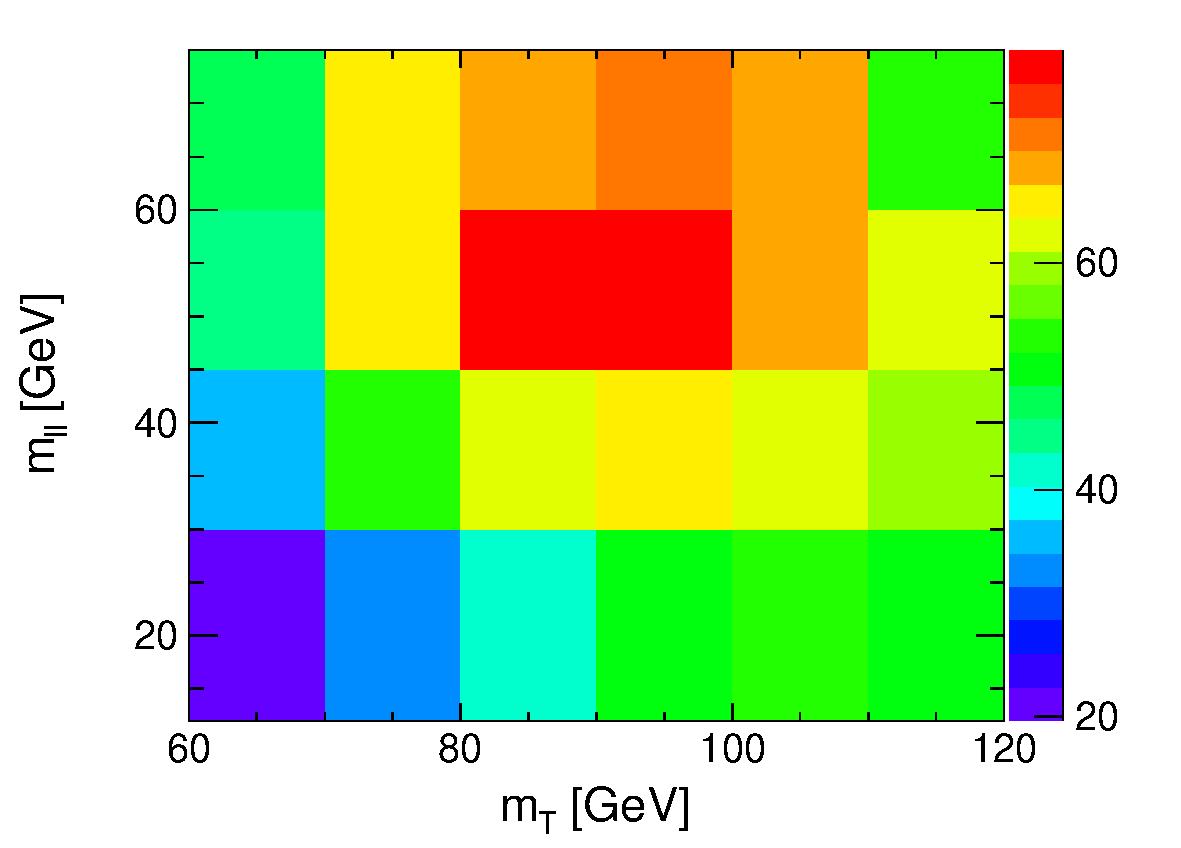
\includegraphics[width=.3\textwidth]{figures/mtvsmll_qqWW_lowmass_0j.pdf}
}
\subfigure[Top]{
\centering
\label{subfig:top_0j}
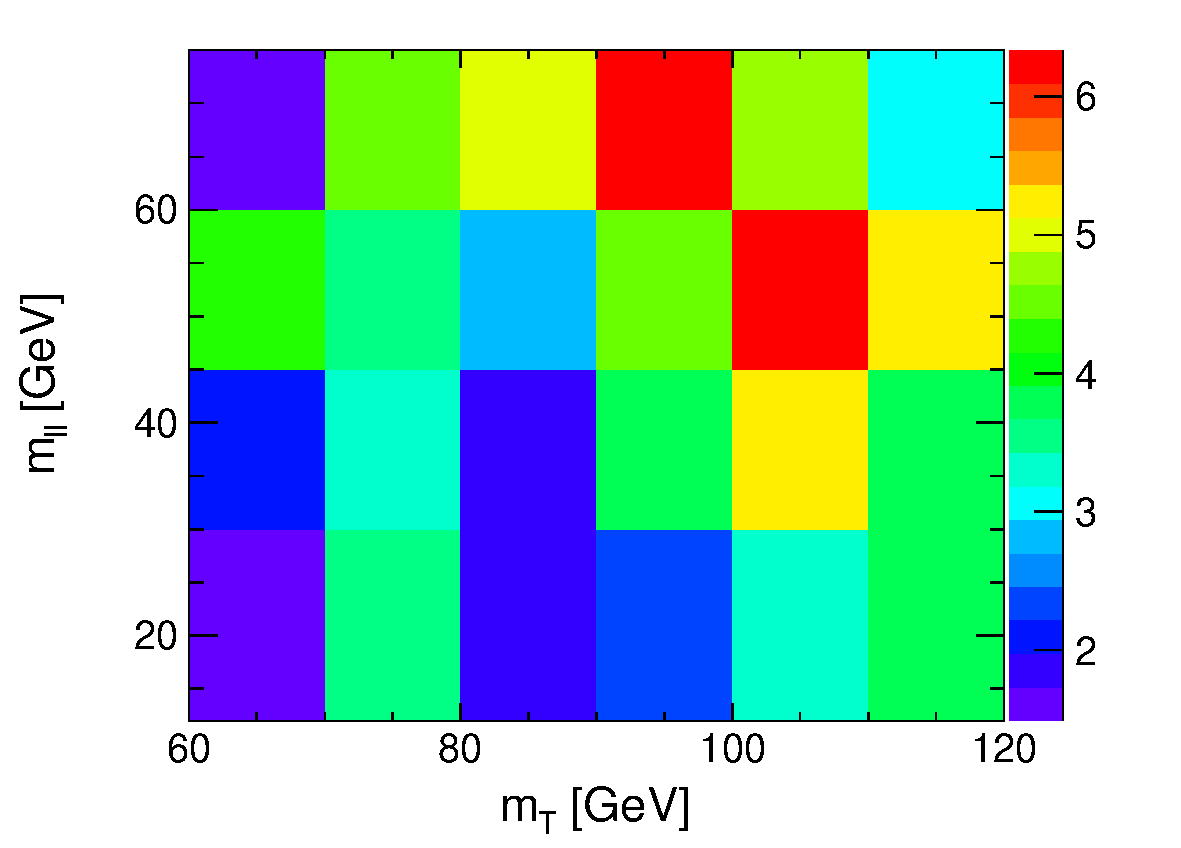
\includegraphics[width=.3\textwidth]{figures/mtvsmll_Top_lowmass_0j.pdf}
} \\ 
\subfigure[Wjets(e)]{
\centering
\label{subfig:wjetse_0j}
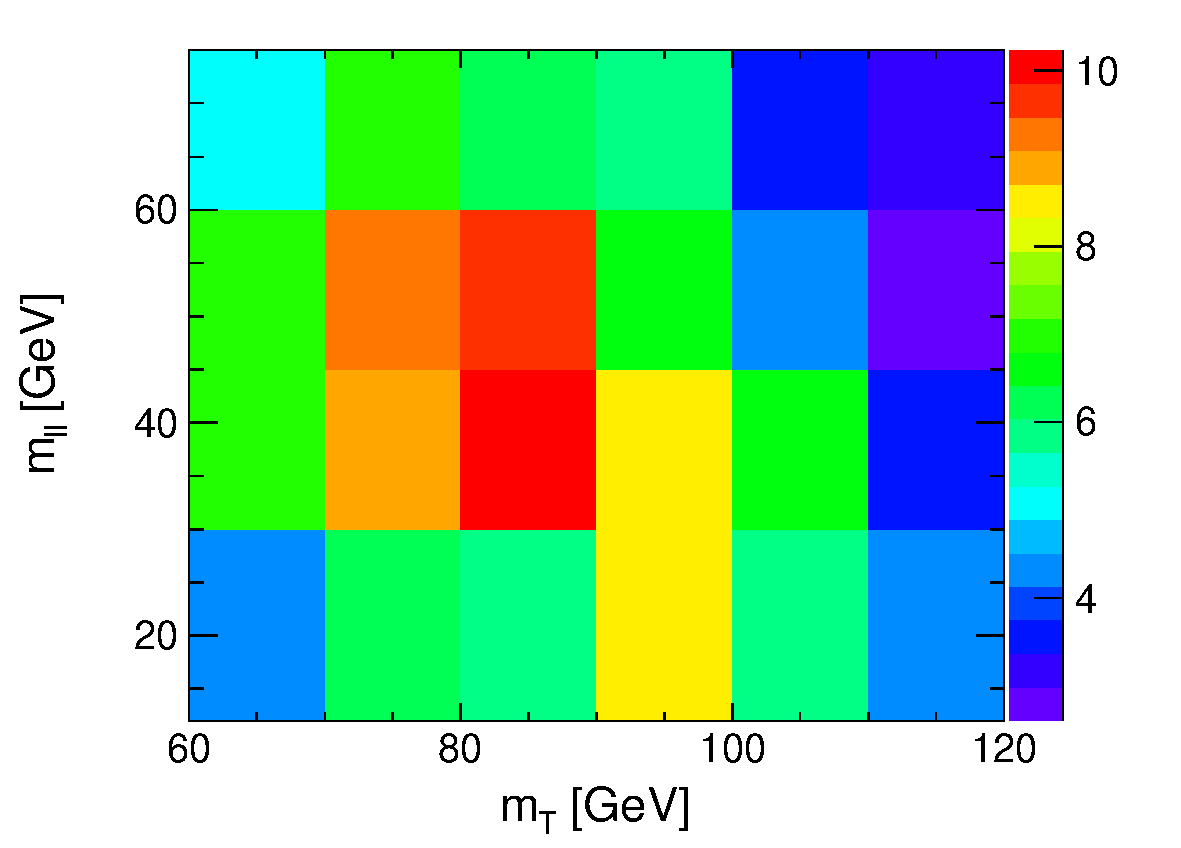
\includegraphics[width=.3\textwidth]{figures/mtvsmll_WjetsE_lowmass_0j.pdf}
}
\subfigure[Wjets($\mu$)]{
\centering
\label{subfig:wjetsm_0j}
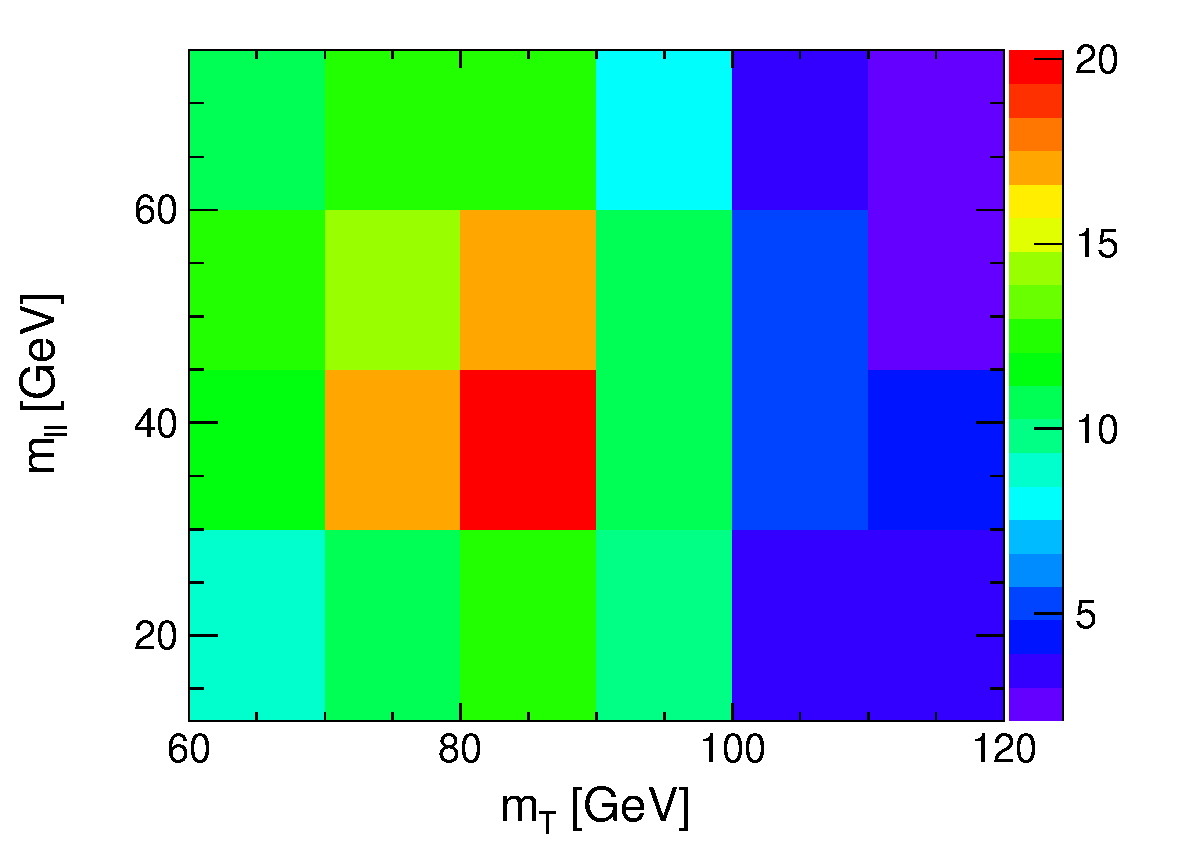
\includegraphics[width=.3\textwidth]{figures/mtvsmll_WjetsM_lowmass_0j.pdf}
} \\
\subfigure[$W\gamma$]{
\centering
\label{subfig:wgamma_0j}
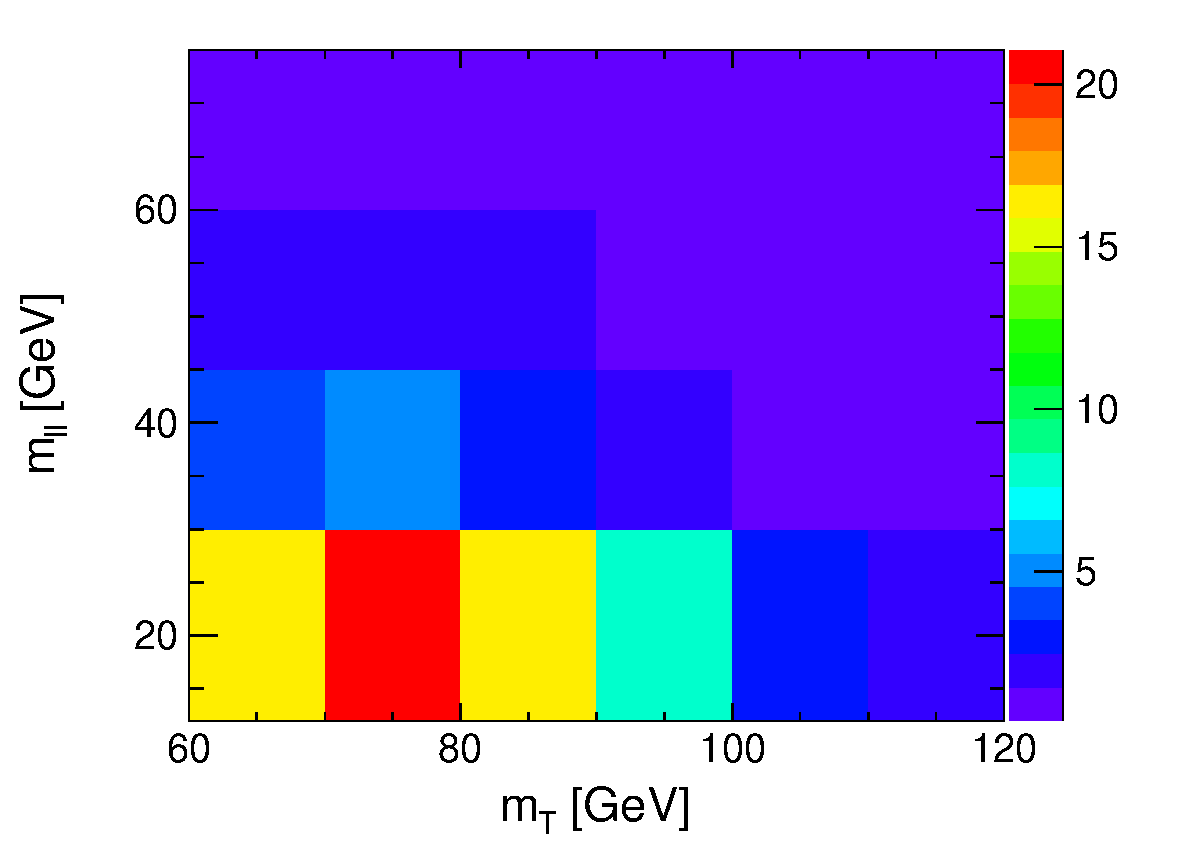
\includegraphics[width=.3\textwidth]{figures/mtvsmll_Wgamma_lowmass_0j.pdf}
} 
\subfigure[$W\gamma^*$]{
\centering
\label{subfig:wgamma_0j}
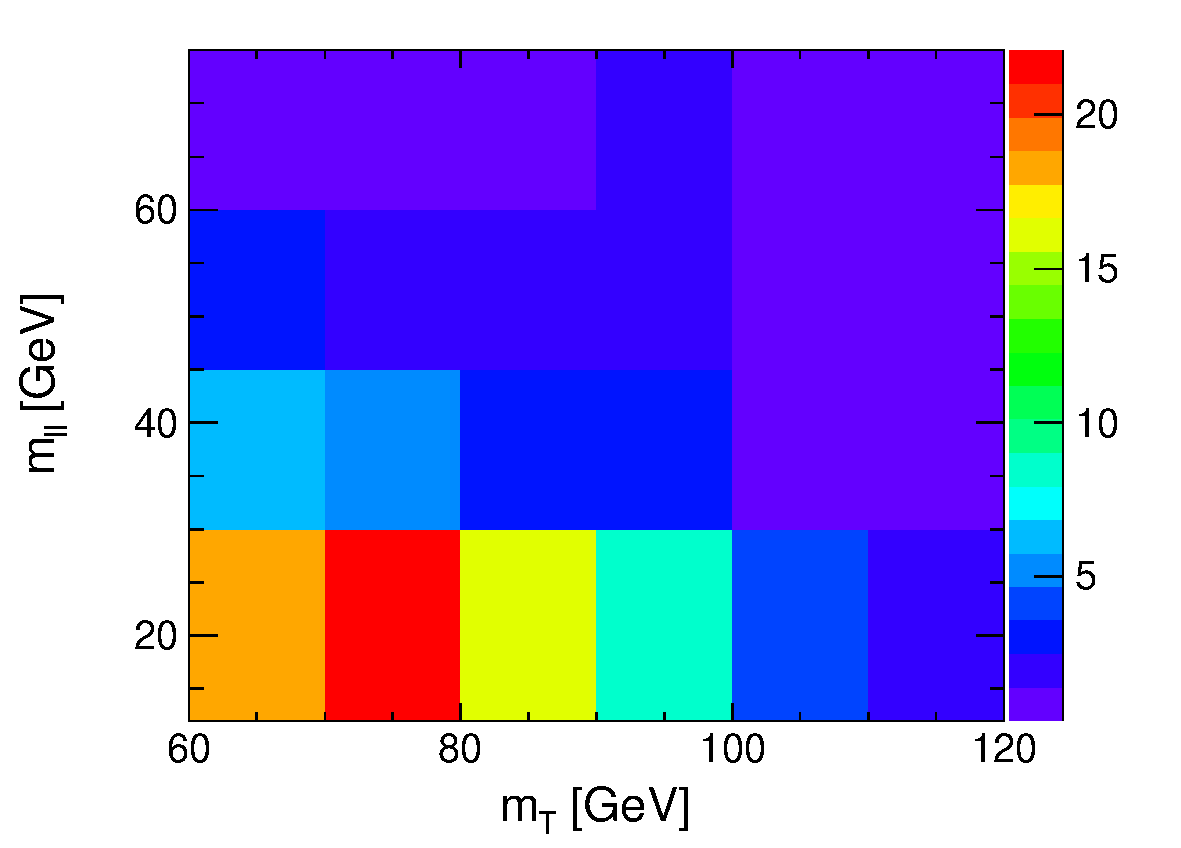
\includegraphics[width=.3\textwidth]{figures/mtvsmll_Wgstar_lowmass_0j.pdf}
} 
\caption{ The 2D ($m_{ll}, m_T$) templates for the main background processes in the 0-Jet with $m_H<300$ GeV.
}
\label{fig:bkg2d_lowmass_0j}
\end{figure}
%%%%%%%%%%%%%%%%%%%%%%%%%%%%%%%


\clearpage

%\subsection{Data templates for $\mHi<300$ GeV} 
%In this section, we show data templates subtracted by background templates. 
%$\mHi=125$ GeV and $\mHi=200$ GeV signal templates are also shown to compare 
%the shapes.

% 0jet
%\begin{figure}[!hbtp]
%\centering
%\subfigure[$\mHi=125$ GeV]{
%\centering
%\label{subfig:m125_0j}
%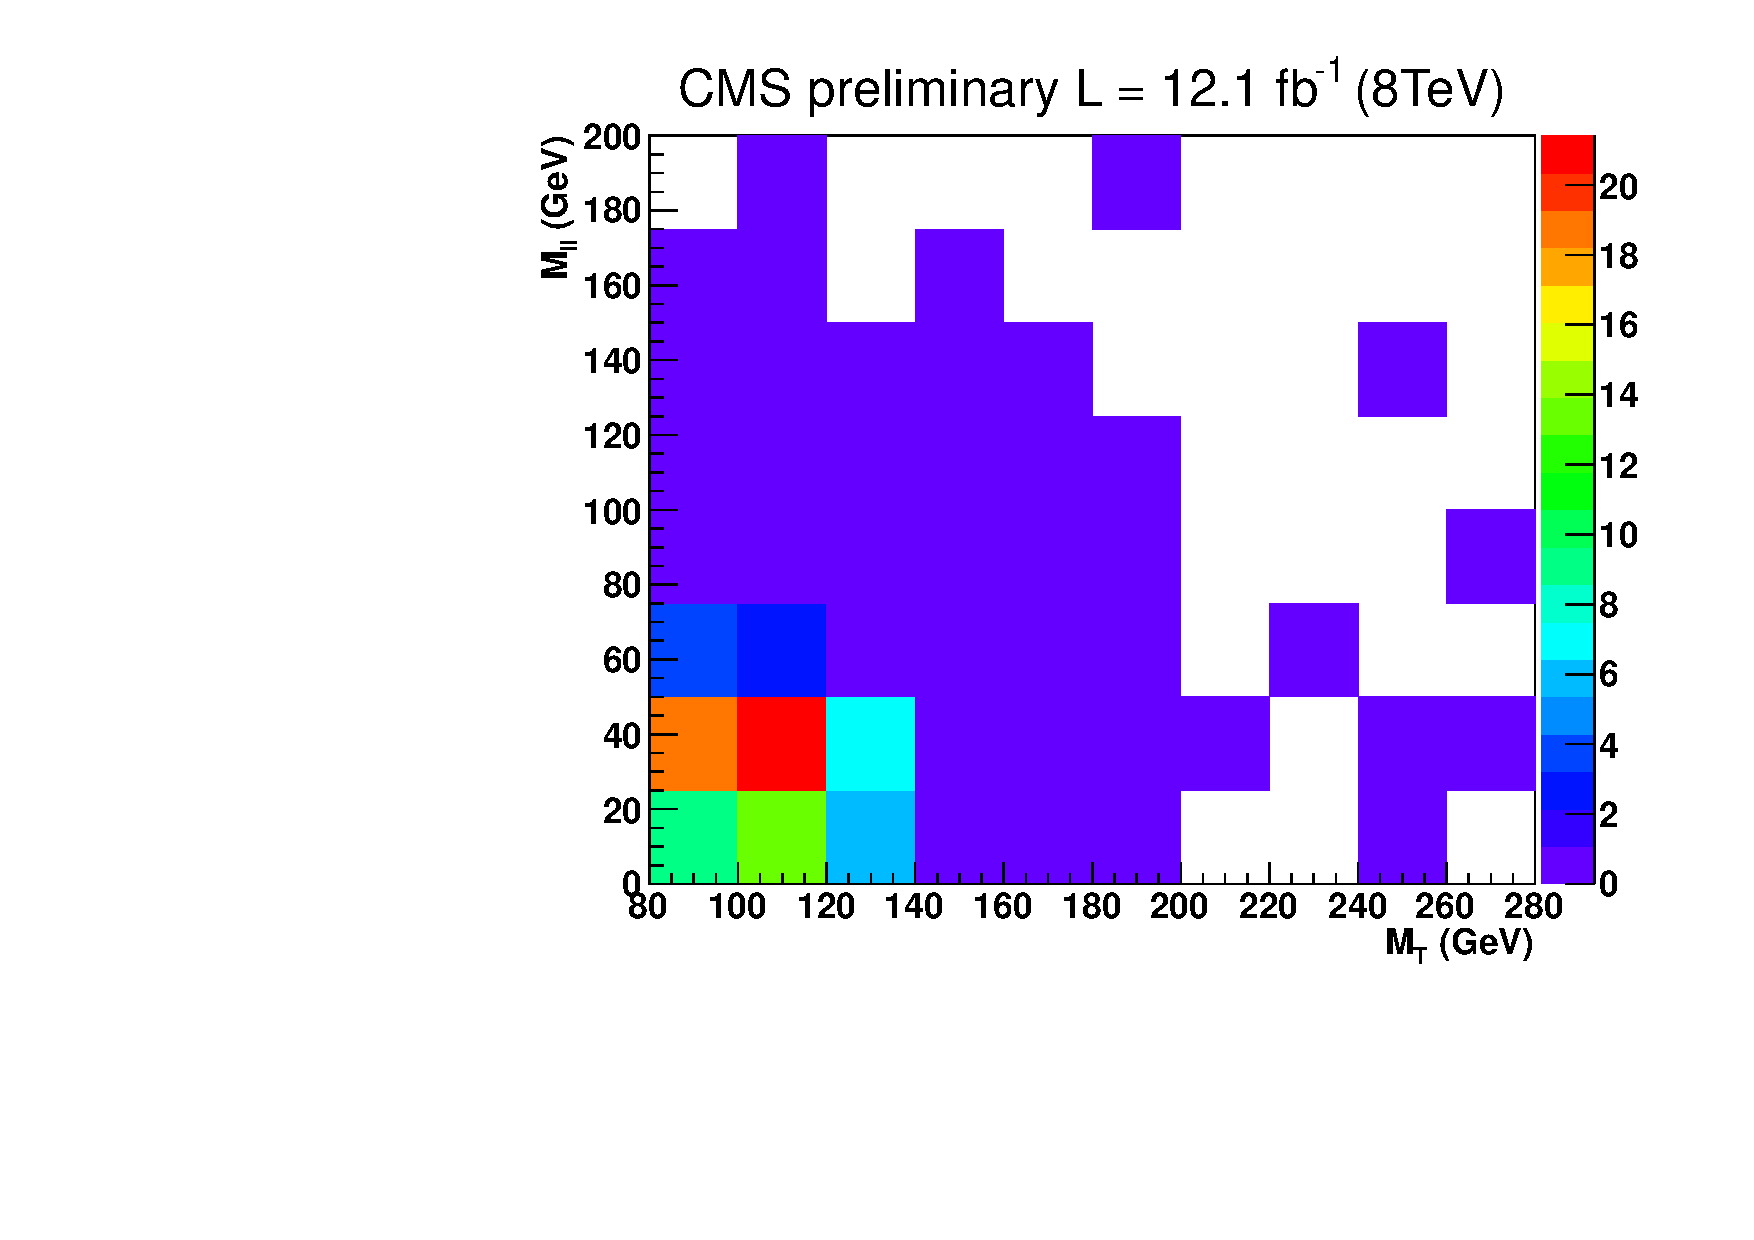
\includegraphics[width=.4\textwidth]{figures/125-0j-2d_prefit_sig_PAS.pdf}
%}
%\subfigure[$\mHi=200$ GeV]{
%\centering
%\label{subfig:m200_0j}
%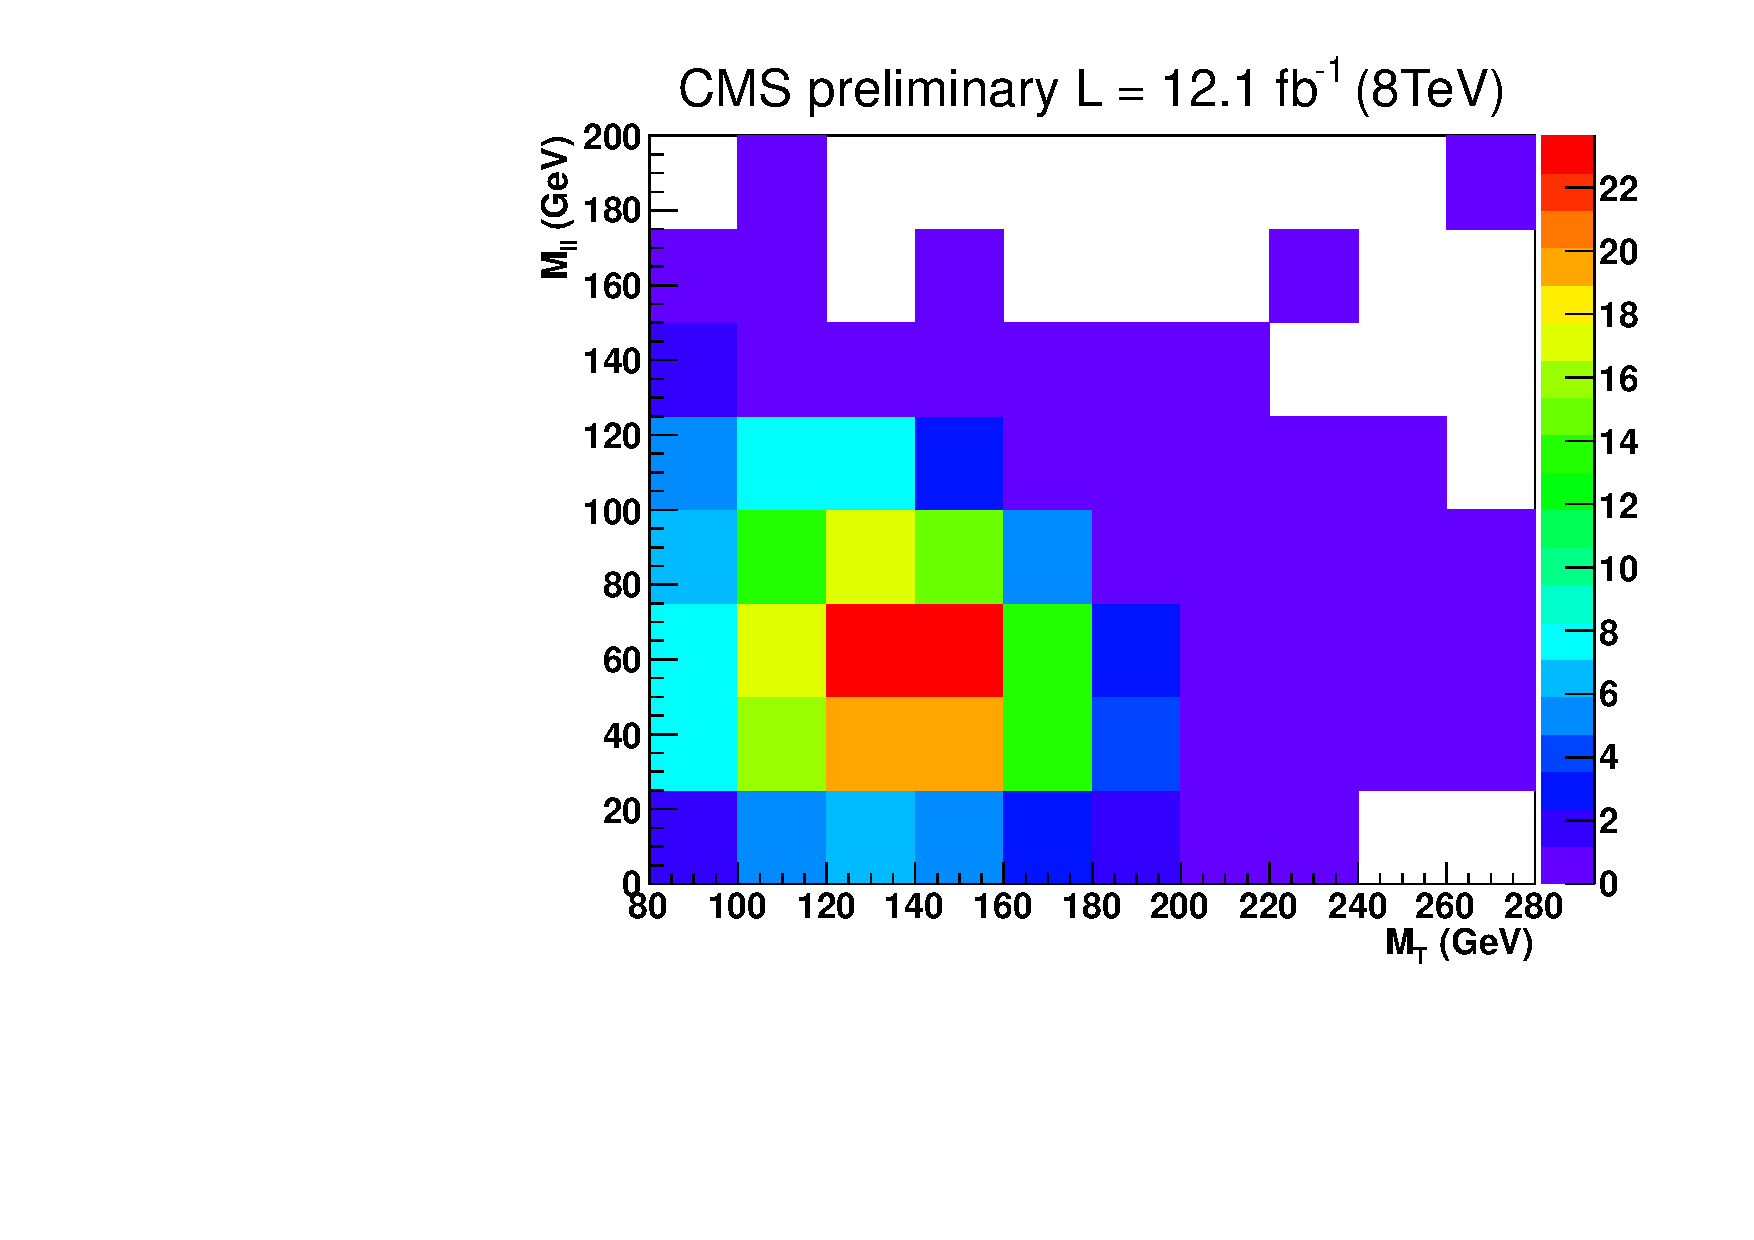
\includegraphics[width=.4\textwidth]{figures/200-0j-2d_prefit_sig_PAS.pdf}
%} \\ 
%\subfigure[Data - background]{
%\centering
%\label{subfig:dataminusbkg_0j}
%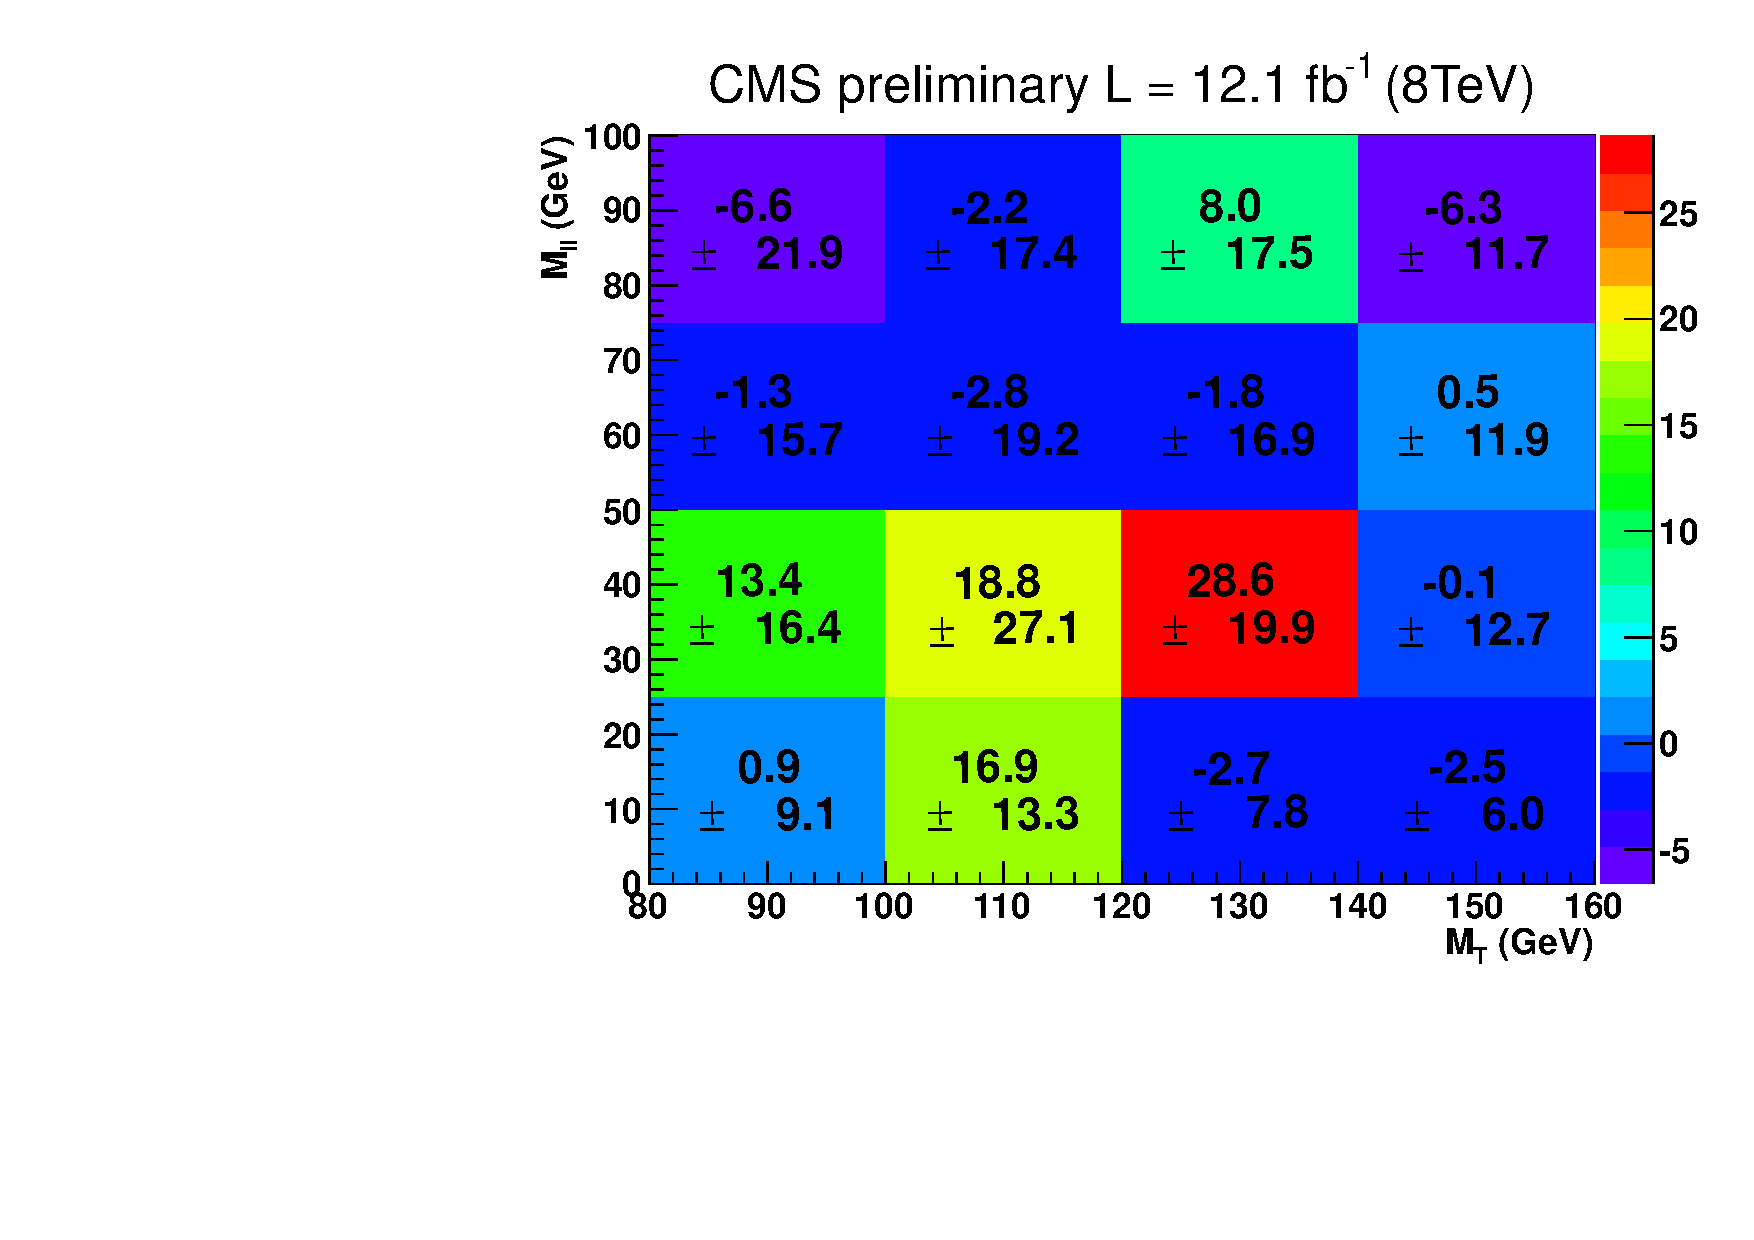
\includegraphics[width=.4\textwidth]{figures/125-0j-2d_postfit_dataminusbkg_PAS.pdf}
%} 
%\caption{ The 2D ($m_{ll}, m_T$) templates for signals($\mHi=125~\GeV$ and $\mHi=200~\GeV$) 
%and data subtracted by backgrounds in the 0-Jet bin. The data templates 
%have the same bin size as used in the analysis, but show only 4x4 bins 
%in low \mt~and \mll~ranges. The uncertainties in the bottom template 
%include statistical uncertainties on data, 
%and statisitical and systematic uncertainties on backgrounds.
%}
%\label{fig:dataminusbkg_0j}
%\end{figure}

% 1jet
%\begin{figure}[!hbtp]
%\centering
%\subfigure[$\mHi=125$ GeV]{
%\centering
%\label{subfig:m125_1j}
%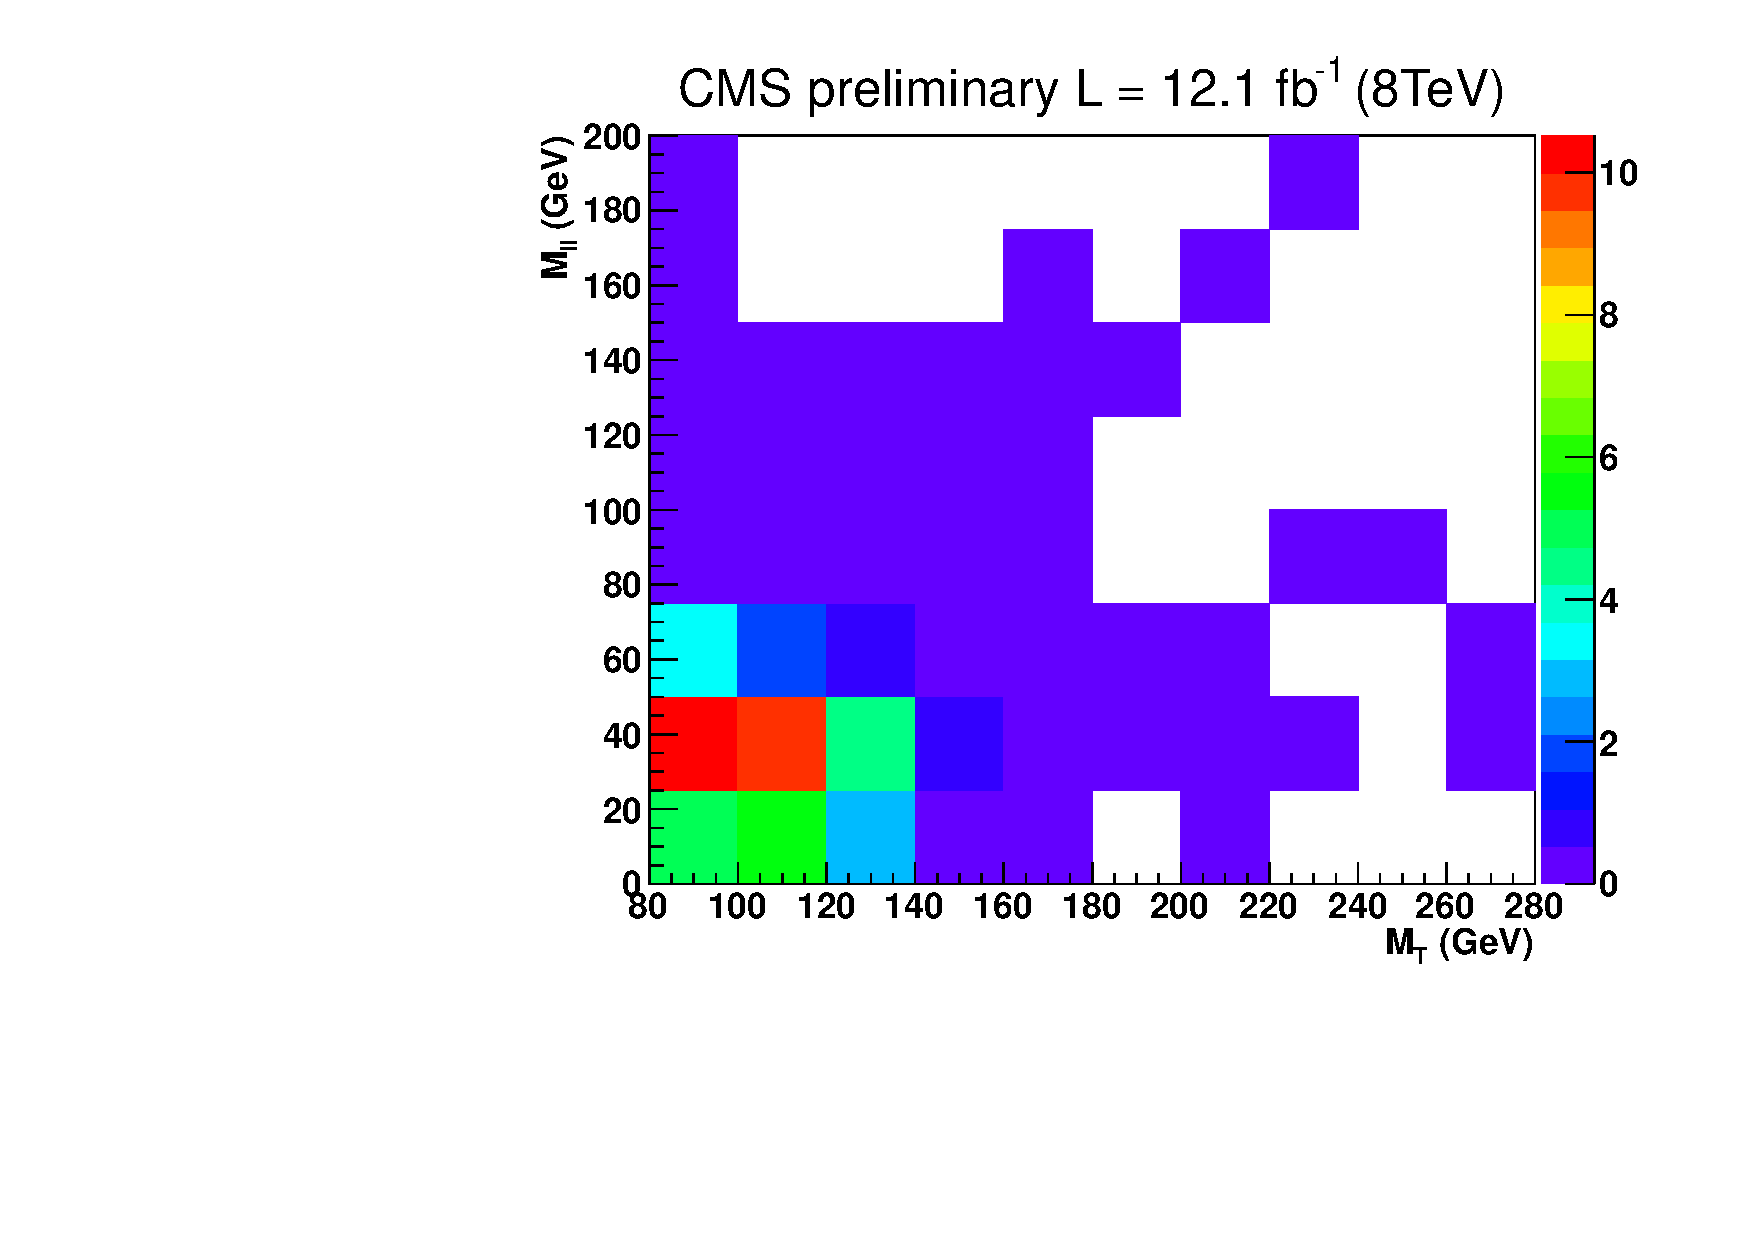
\includegraphics[width=.4\textwidth]{figures/125-1j-2d_prefit_sig_PAS.pdf}
%}
%\subfigure[$\mHi=200$ GeV]{
%\centering
%\label{subfig:m200_1j}
%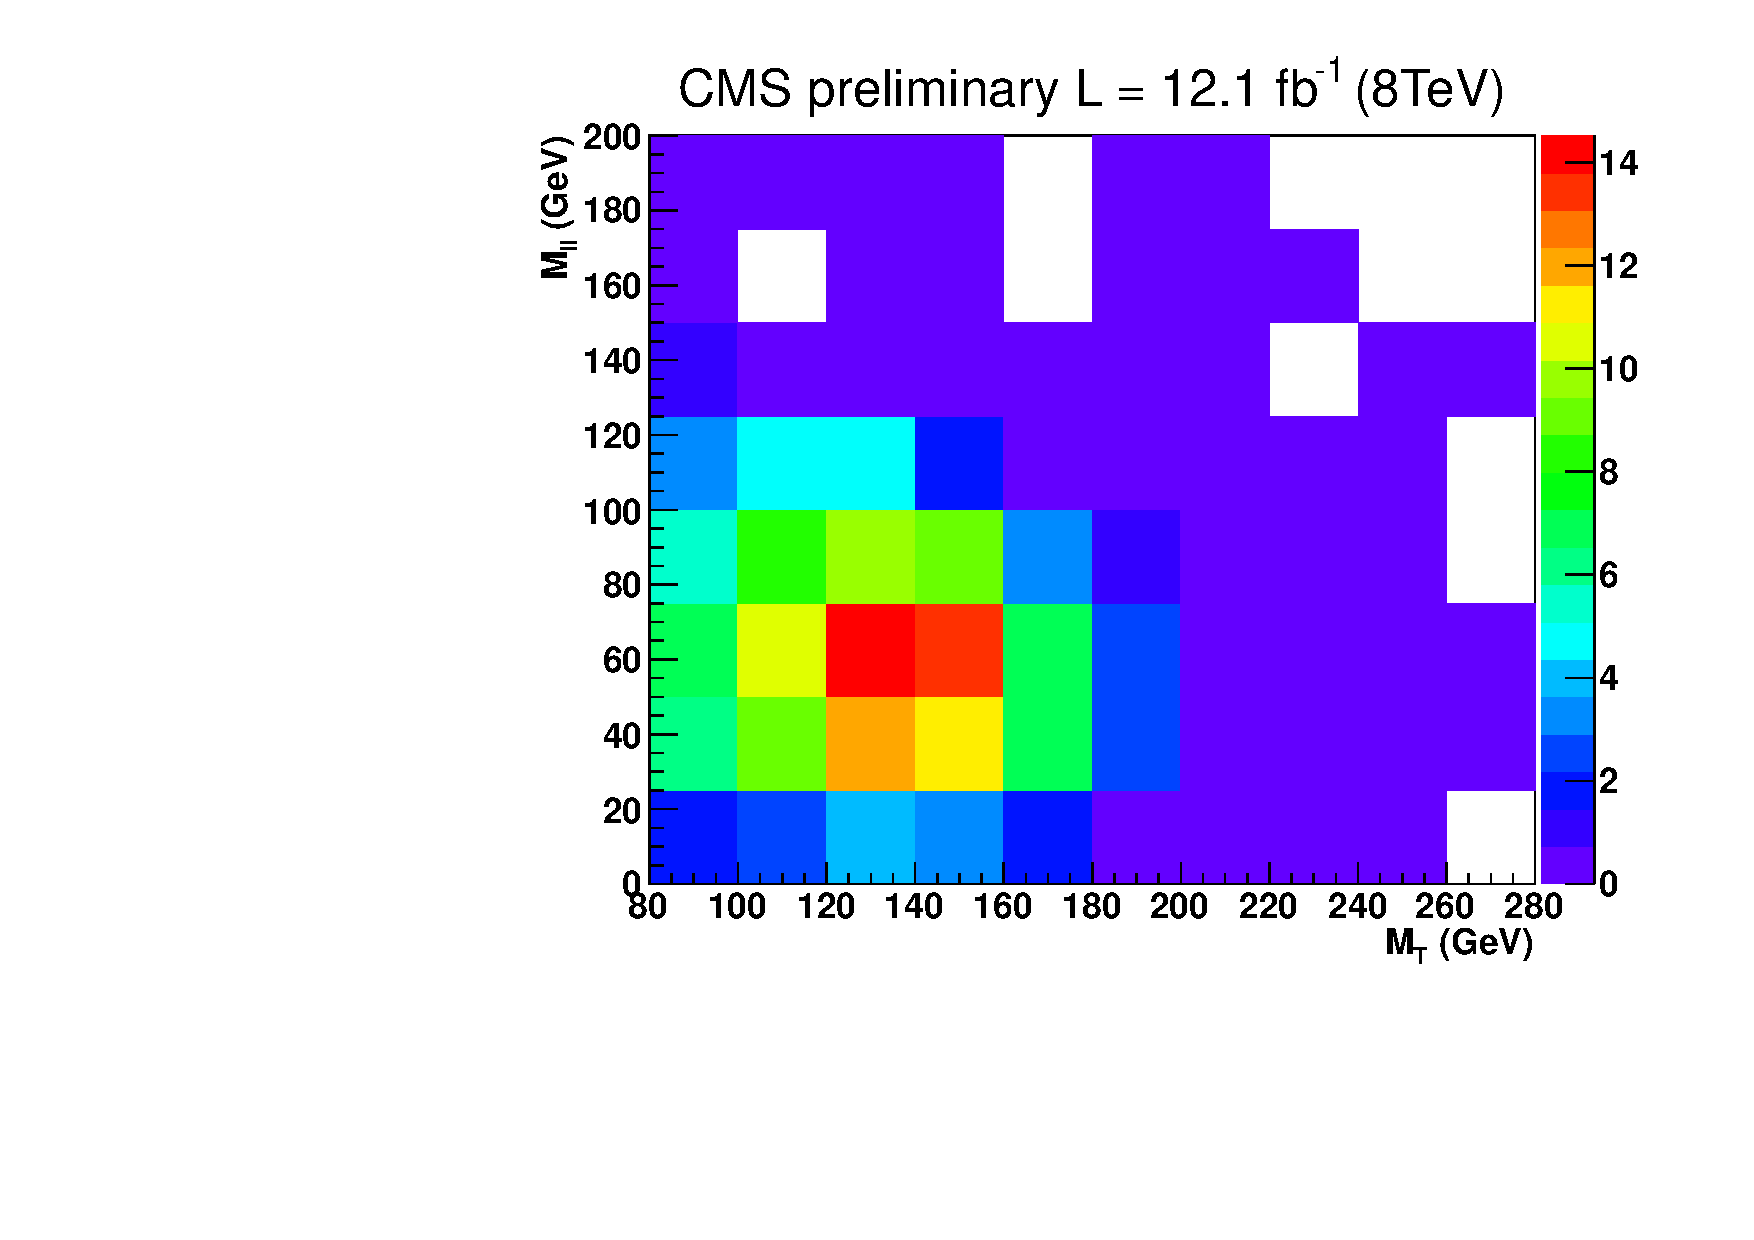
\includegraphics[width=.4\textwidth]{figures/200-1j-2d_prefit_sig_PAS.pdf}
%} \\ 
%\subfigure[Data - background]{
%\centering
%\label{subfig:dataminusbkg_1j}
%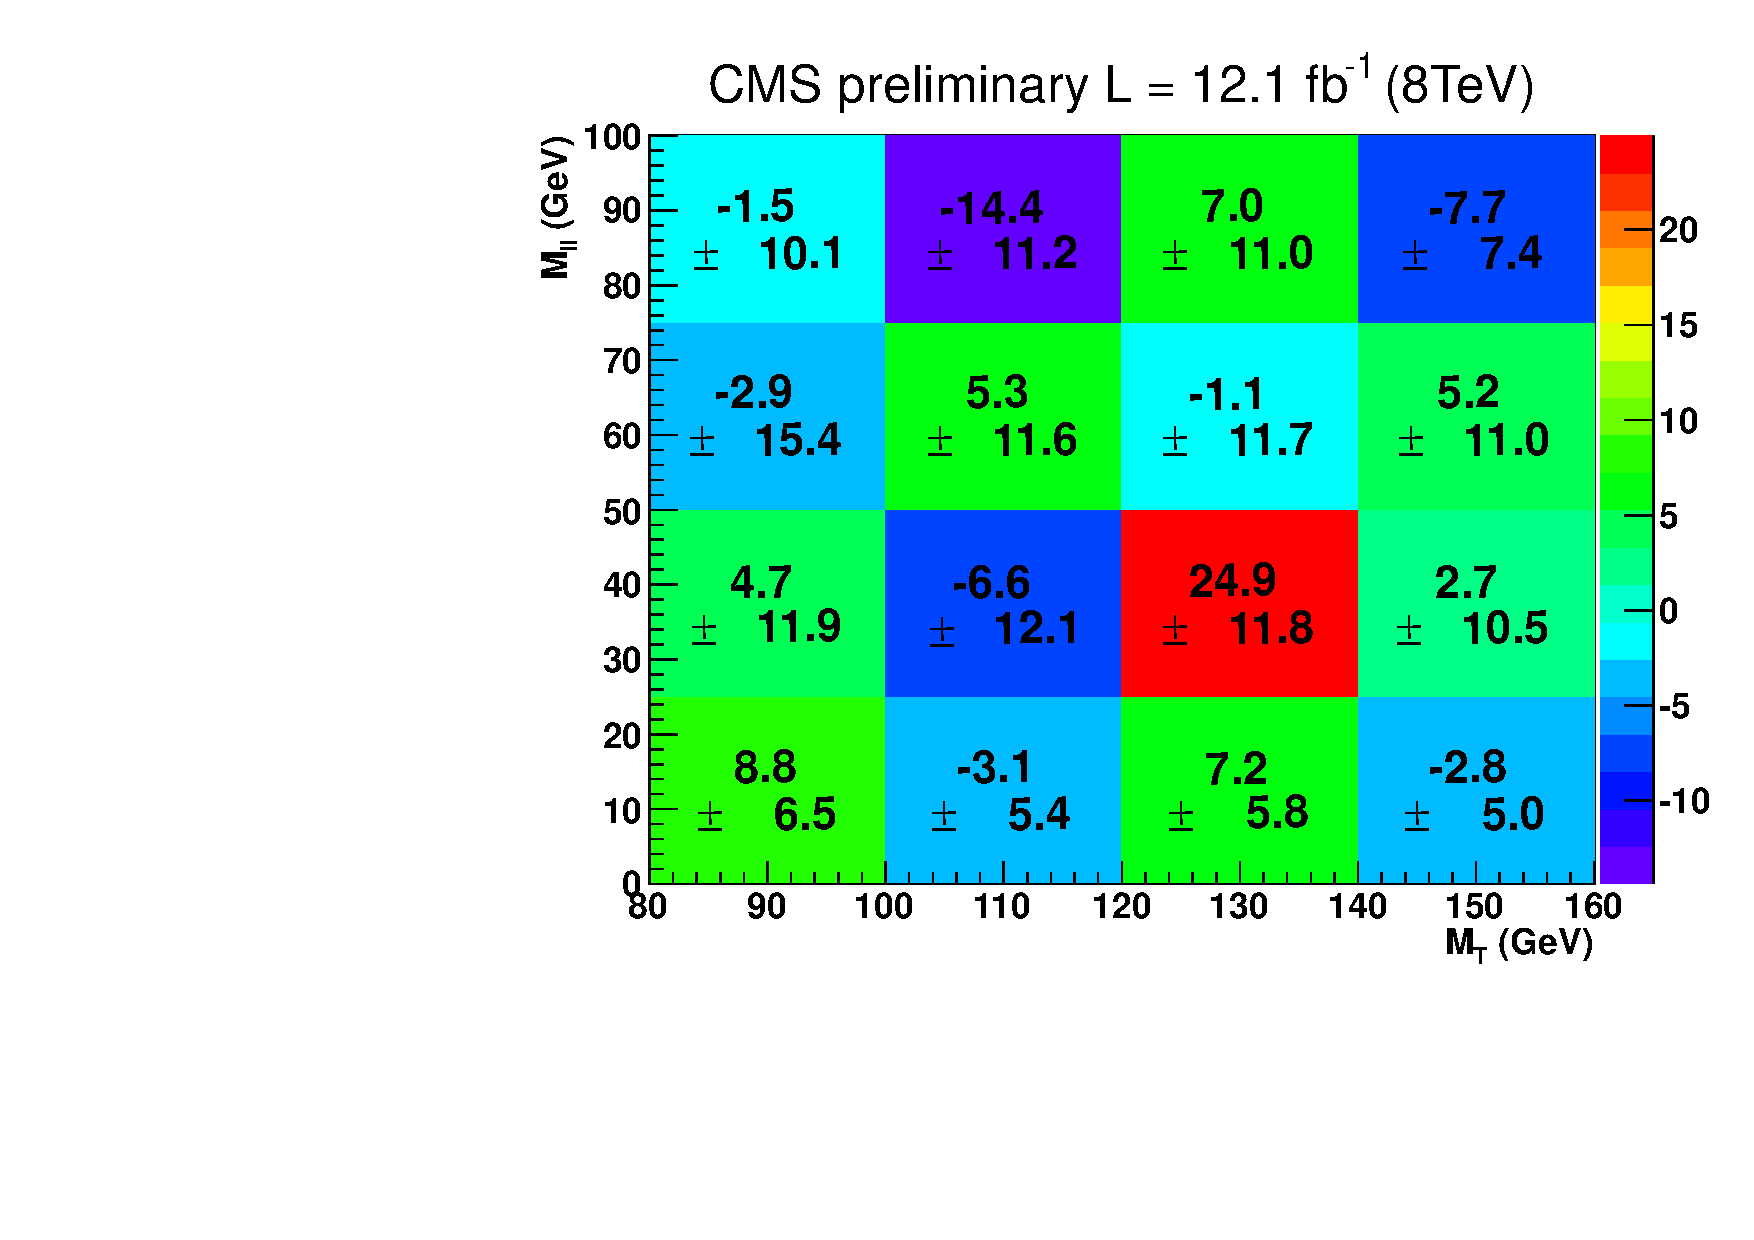
\includegraphics[width=.4\textwidth]{figures/125-1j-2d_postfit_dataminusbkg_PAS.pdf}
%} 
%\caption{ The 2D ($m_{ll}, m_T$) templates for signals($\mHi=125~\GeV$ and $\mHi=200~\GeV$) 
%and data subtracted by backgrounds in the 1-Jet bin. The data templates 
%have the same bin size as used in the analysis, but show only 4x4 bins 
%in low \mt~and \mll~ranges. The uncertainties in the bottom template 
%include statistical uncertainties on data, 
%and statisitical and systematic uncertainties on backgrounds.
%}
%\label{fig:dataminusbkg_1j}
%\end{figure}

